\documentclass[11pt, letterpaper]{article}
\usepackage[utf8]{inputenc}
\usepackage{geometry}
\usepackage{fancyhdr}
\usepackage{amsmath, amssymb}
\usepackage{xcolor}
\usepackage{listings}
\usepackage{enumitem}
\usepackage{hyperref}
\usepackage{booktabs}
\usepackage{graphicx}
\newcommand{\E}{\mathbb{E}}
\newcommand{\Var}{\mathrm{Var}}

\setlength{\parindent}{0pt}
\setlist{itemsep=0.5em}
\setlength{\parskip}{0.5em}

\geometry{margin=1in}
\pagestyle{fancy}
\fancyhf{}
\lhead{\textbf{Solutions}}
\rhead{\textbf{Data Analysis and Regression, Homework 3}}
\cfoot{\thepage}

\definecolor{codegreen}{rgb}{0,0.6,0}
\definecolor{codegray}{rgb}{0.5,0.5,0.5}
\definecolor{codepurple}{rgb}{0.58,0,0.82}
\definecolor{backcolour}{rgb}{0.95,0.95,0.92}

\lstdefinestyle{mystyle}{
    backgroundcolor=\color{backcolour},   
    commentstyle=\color{codegreen},
    keywordstyle=\color{magenta},
    numberstyle=\tiny\color{codegray},
    stringstyle=\color{codepurple},
    basicstyle=\ttfamily\footnotesize,
    breakatwhitespace=false,         
    breaklines=true,                 
    captionpos=b,                    
    keepspaces=true,                 
    numbers=left,                    
    numbersep=5pt,                  
    showspaces=false,                
    showstringspaces=false,
    showtabs=false,                  
    tabsize=2
}
\lstset{style=mystyle}

\newcommand{\problem}[1]{\section*{Problem #1}}
\newcommand{\subproblem}[1]{\subsection*{Problem #1}}
\newcommand{\answer}{\textbf{\textit{\textcolor{red}{Answer:}}}\\}

\begin{document}

\section*{Instructions}
\begin{itemize}
    \item Homework 3 was due Monday, August 10th at 18:00 Chicago Time.
    \item All numbers and figures come from \texttt{homework\_3\_solution.ipynb}, run from top to bottom.
\end{itemize}
\hrule
\vspace{0.5cm}

\pagebreak

\problem{1: Ridge Regression and Stability}

Generate a dataset with $n=100$ observations based on the true model:
$$ y = 1 + x_1 + x_2 + \epsilon $$
where $\epsilon \sim \mathcal{N}(0, 1)$.

Additionally, make $x_1, x_2 \sim \mathcal{N}(0, 1)$ highly correlated, with $\rho = 0.99999$. You
can do this via the following code snippet:
    \begin{lstlisting}[language=Python]
import numpy as np
np.random.seed(1)

mean = [0, 0]
cov = [[1, 0.99999], [0.99999, 1]]
x1, x2 = np.random.multivariate_normal(mean, cov, 100).T
epsilon = np.random.normal(0, 1, 100)\end{lstlisting}
    


\subproblem{1.1: OLS Inference}
Fit an OLS model to your generated data using \texttt{statsmodels}.
\begin{itemize}
    \item Report the p-values and confidence intervals for $\hat{\beta}_1$ and $\hat{\beta}_2$.
    \item Discuss the results. Are the coefficients close to the true values ($1$ and $1$)? Are they statistically significant?
\end{itemize}

\answer
$R^2 = 0.733$.

\begin{center}
\begin{tabular}{lcccccc}
\toprule
               & \textbf{coef} & \textbf{std err} & \textbf{t} & \textbf{P$> |$t$|$} & \textbf{[0.025} & \textbf{0.975]}  \\
\midrule
\textbf{const} &       0.9940  &        0.105     &     9.483  &         0.000        &        0.786    &        1.202     \\
\textbf{X1}    &      24.1321  &       24.274     &     0.994  &         0.323        &      -24.046    &       72.310     \\
\textbf{X2}    &     -22.1958  &       24.257     &    -0.915  &         0.362        &      -70.340    &       25.948     \\
\bottomrule
\end{tabular}
\end{center}

Neither slope is close to $1$, and neither is significant: $p = 0.323$ and $p = 0.362$, with
intervals almost $100$ units wide. Yet the intercept is estimated precisely and $R^2 = 0.733$, so
the model as a whole fits.

That is multicollinearity. With $\rho = 0.99999$ the data cannot separate $\beta_1$ from $\beta_2$,
only their sum, and $\hat{\beta}_1 + \hat{\beta}_2 = 1.94$ against a true sum of $2$.


\subproblem{1.2: Stability}
Now, re-generate your data using \texttt{np.random.seed(42)} and fit the OLS model again.
\begin{itemize}
    \item Report the new estimates for $\hat{\beta}_1$ and $\hat{\beta}_2$.
    \item Compare these estimates to the previous ones. What do you notice?
\end{itemize}

\answer
\begin{center}
\begin{tabular}{lcccccc}
\toprule
               & \textbf{coef} & \textbf{std err} & \textbf{t} & \textbf{P$> |$t$|$} & \textbf{[0.025} & \textbf{0.975]}  \\
\midrule
\textbf{const} &       1.0928  &        0.108     &    10.115  &         0.000        &        0.878    &        1.307     \\
\textbf{X1}    &      39.3968  &       24.079     &     1.636  &         0.105        &       -8.393    &       87.187     \\
\textbf{X2}    &     -37.5875  &       24.083     &    -1.561  &         0.122        &      -85.386    &       10.211     \\
\bottomrule
\end{tabular}
\end{center}

Changing the seed moves $\hat{\beta}_1$ from $24.13$ to $39.40$ and $\hat{\beta}_2$ from $-22.20$
to $-37.59$. The individual coefficients are not reproducible at all.

The sums are close: $1.94$ before, $1.81$ now. Only the sum is identified.


\subproblem{1.3 Variance via Simulation}

To better understand this phenomenon, run a simulation (note, you will need to unset the random seed for this part):
\begin{itemize}
    \item Run a simulation loop 1000 times. In each iteration, generate a new dataset ($x1, x2, \epsilon$) and fit an OLS model.
    \item Store the estimates for $\hat{\beta}_1$ and $\hat{\beta}_2$.
\end{itemize}
Plot 2 histograms showing the distribution of the estimates for $\hat{\beta}_1$ and $\hat{\beta}_2$.
Additionally, report the volatility (standard deviation) of your $\hat{\beta}_1$ and $\hat{\beta}_2$ estimates across the simulations.

\answer
\begin{center}
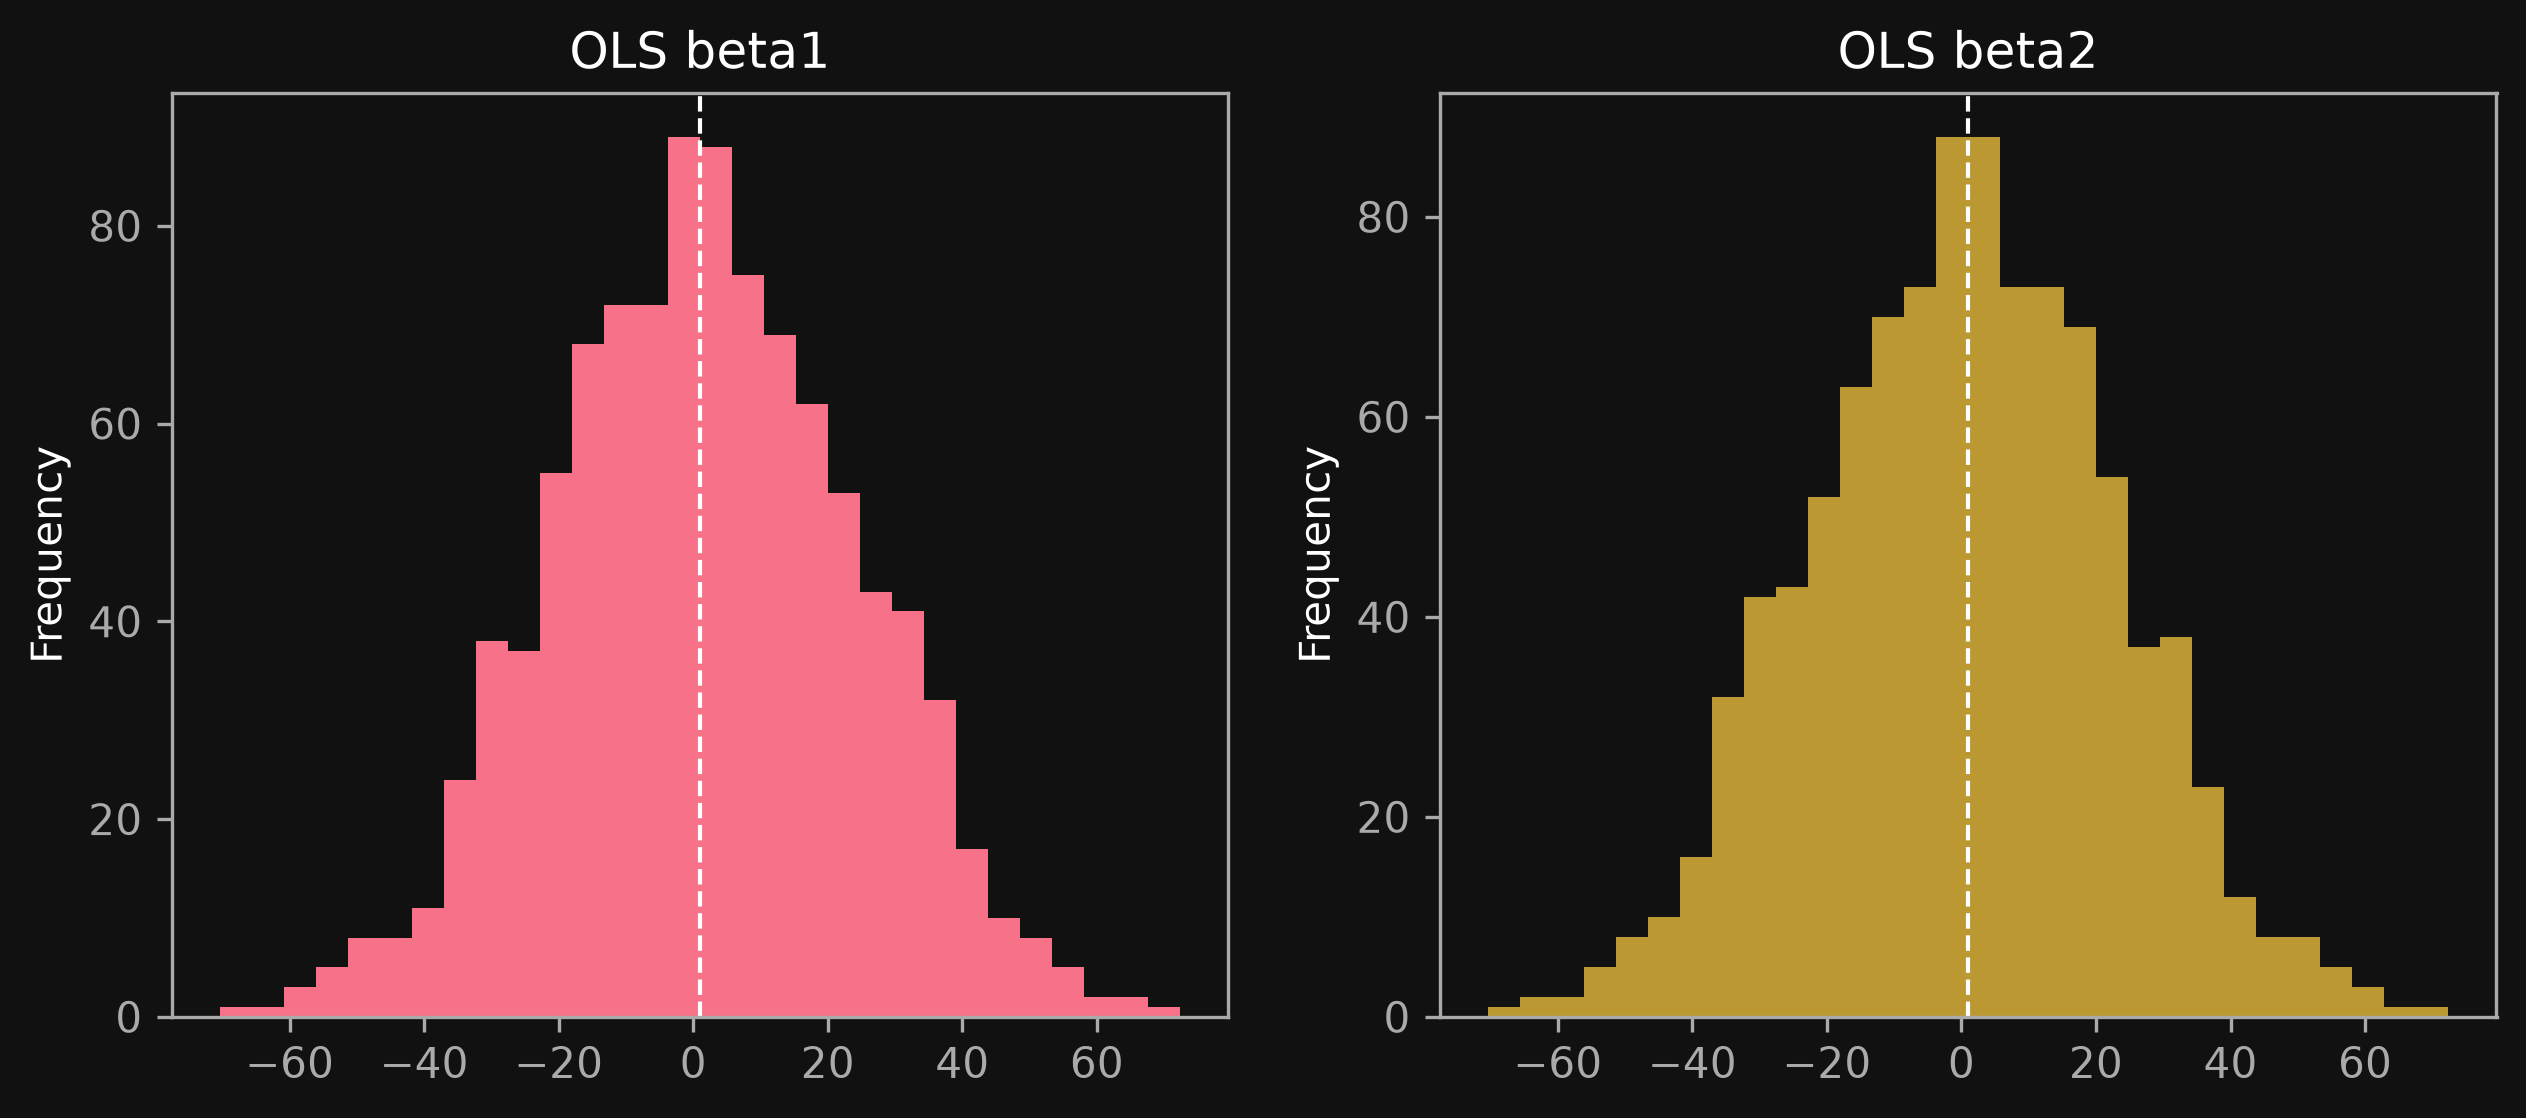
\includegraphics[width=0.95\textwidth]{./figures/problem1_simulation_histograms.png}
\end{center}

Standard deviation across the 1000 fits: $22.4496$ for $\hat{\beta}_1$ and $22.4495$ for
$\hat{\beta}_2$, against a true value of $1$ for each. The two histograms are mirror images because
the errors cancel: $\hat{\beta}_1$ and $\hat{\beta}_2$ are almost perfectly negatively correlated,
so their sum stays near $2$ while each one wanders with a standard deviation of $22$.


\subproblem{1.3: Ridge to the Rescue}
Now, fit a Ridge Regression model using \texttt{statsmodels} (you can use \texttt{fit\_regularized} with \texttt{L1\_wt=0} for Ridge).
\begin{itemize}
    \item Use three different values for alpha (lambda): $0.01$, $0.1$, and $1$.
    \item For each alpha, report the coefficients $\hat{\beta}_1$ and $\hat{\beta}_2$.
    \item Discuss how the coefficients change with different alpha values.
\end{itemize}

\answer
Fitted on the seed-1 dataset from 1.1, so these are directly comparable to the $24.13$ and $-22.20$
reported there.

\begin{center}
\begin{tabular}{rrrr}
\toprule
$\alpha$ & const & X1 & X2 \\
\midrule
0.01 & 0.9784 & \textbf{0.9720} & \textbf{0.9324} \\
0.10 & 0.8713 & 0.8883 & 0.8850 \\
1.00 & 0.3997 & 0.5358 & 0.5358 \\
\bottomrule
\end{tabular}
\end{center}

A penalty of $0.01$ is enough. The coefficients go from $24.13$ and $-22.20$ to $0.9720$ and
$0.9324$, both within $7\%$ of the truth.

The penalty breaks the tie between the two collinear columns. OLS is free to put a huge positive
weight on one and cancel it with a huge negative weight on the other, because the residual sum of
squares barely notices; ridge charges $\alpha \|\beta\|^2$ for that, so the cheapest way to produce
the same fitted values is to split the effect evenly. Numerically, this is the same statement as
$X^\top X + \alpha I$ being far better conditioned than $X^\top X$.

Past that point $\alpha$ costs accuracy: by $\alpha = 1$ both coefficients have been shrunk to
$0.5358$ and the intercept to $0.3997$.


\subproblem{1.4: Ridge Simulation}
Next, you should repeat the simulation from subproblem 1.3, but this time use a Ridge model with a fixed alpha of $0.01$.
\begin{itemize}
    \item Run the simulation loop 1000 times, generating new datasets and fitting the Ridge model each time.
    \item Store the estimates for $\hat{\beta}_1$ and $\hat{\beta}_2$.
\end{itemize}
Plot 2 histograms showing the distribution of the Ridge estimates for $\hat{\beta}_1$ and $\hat{\beta}_2$.
Additionally, report the volatility (standard deviation) of your Ridge $\hat{\beta}_1$ and $\hat{\beta}_2$ estimates across the simulations.
Compare these volatilities to those obtained from the OLS simulation in subproblem 1.3.

\answer
\begin{center}
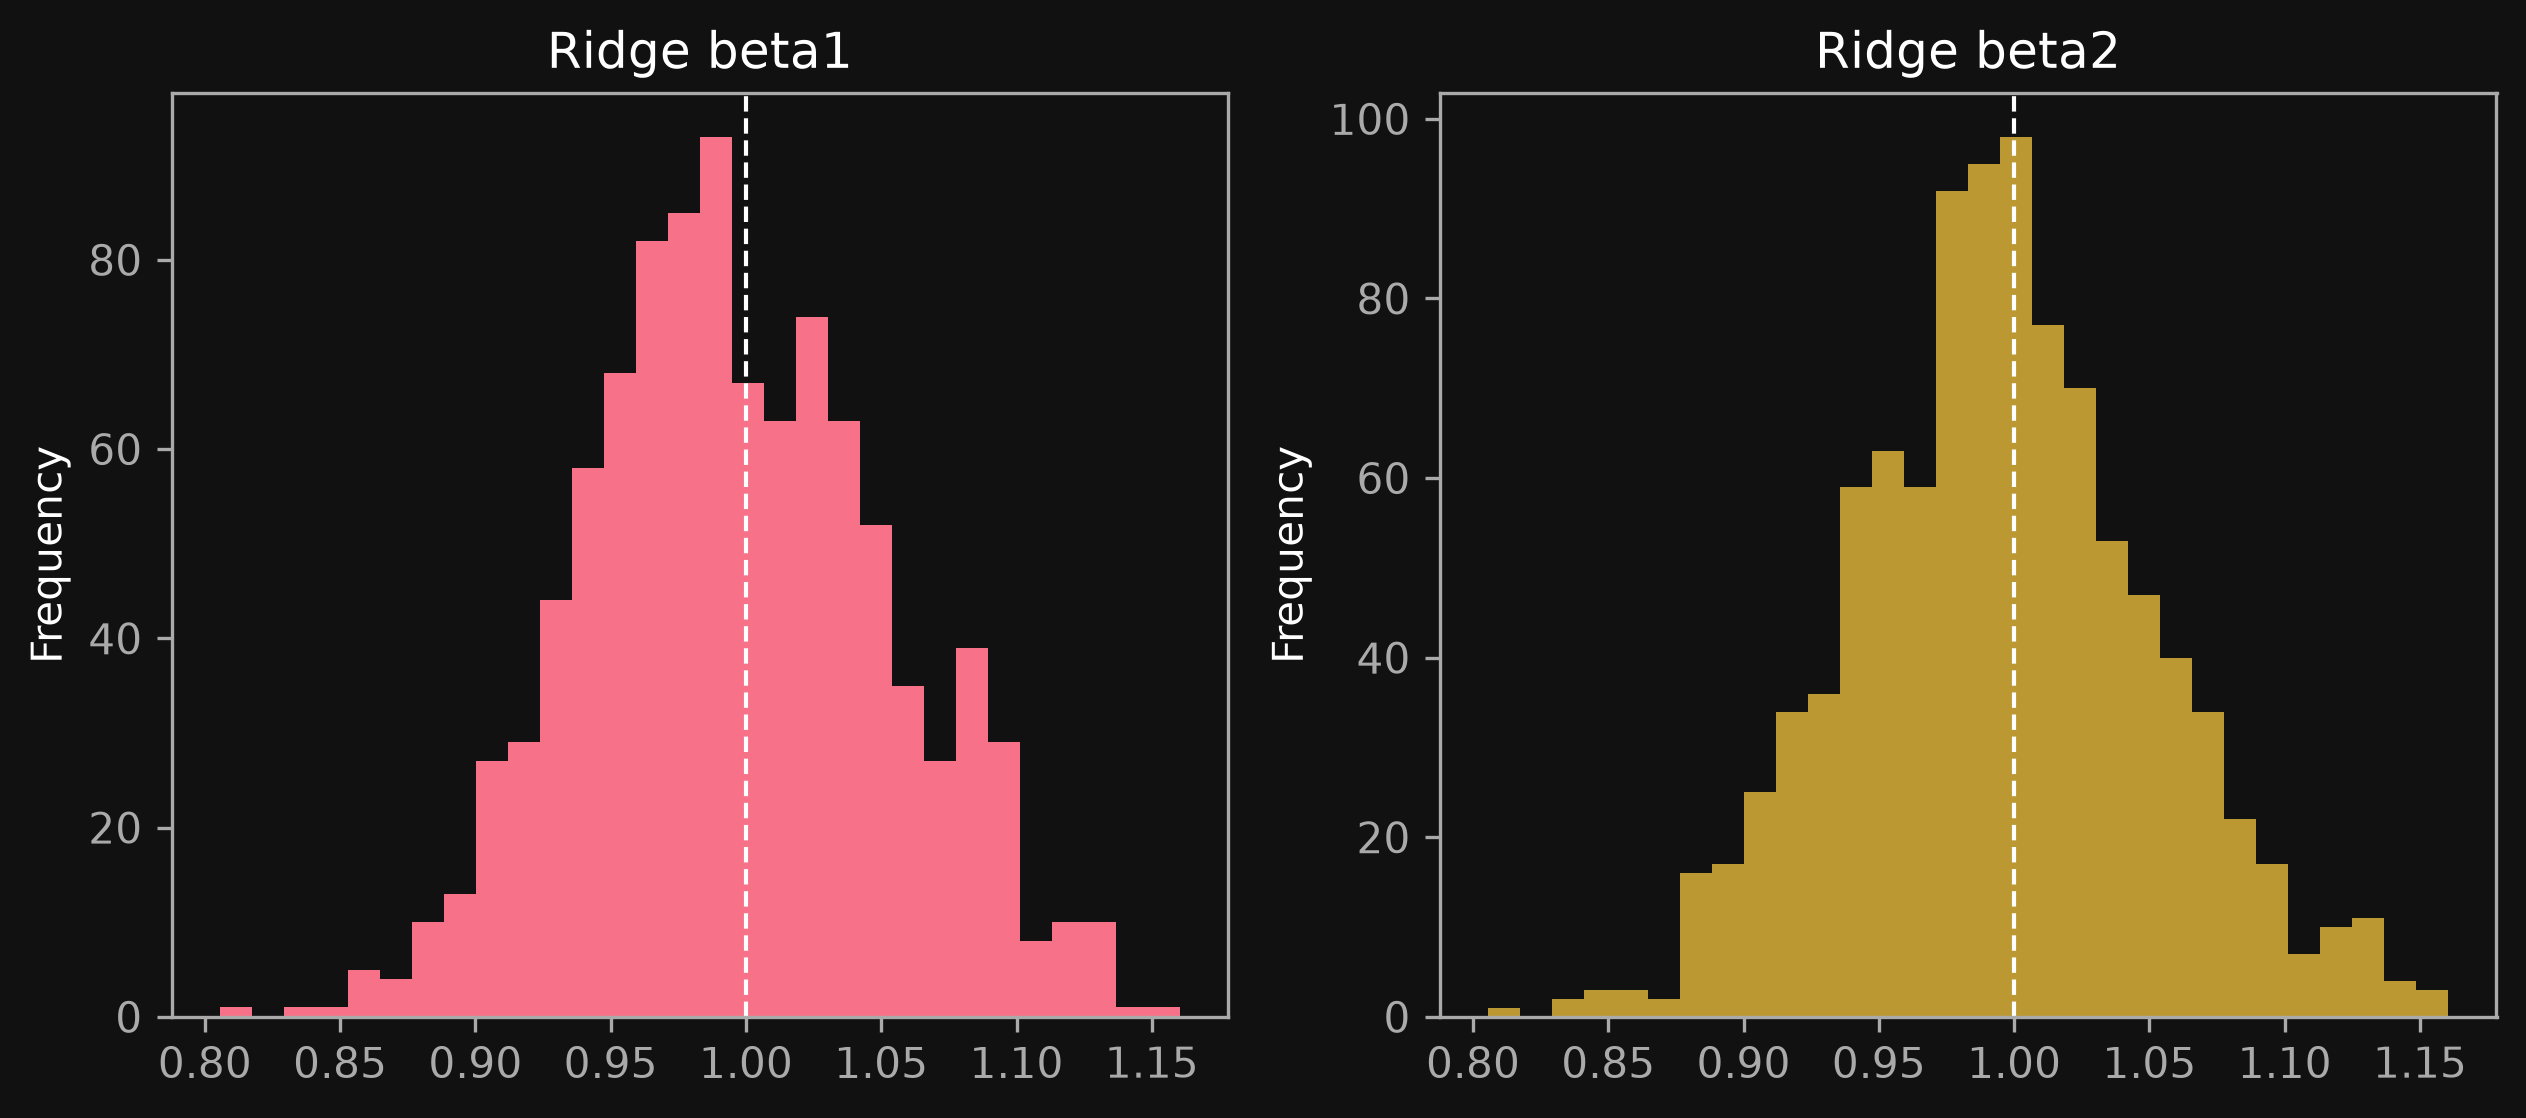
\includegraphics[width=0.95\textwidth]{./figures/problem1_ridge_histograms.png}
\end{center}

\begin{center}
\begin{tabular}{lrr}
\toprule
 & OLS & Ridge ($\alpha = 0.01$) \\
\midrule
sd($\hat{\beta}_1$) & 22.4496 & 0.0563 \\
sd($\hat{\beta}_2$) & 22.4495 & 0.0562 \\
\bottomrule
\end{tabular}
\end{center}

Both simulations use the same seed, so they run on identical datasets. A penalty of $0.01$ cuts the
volatility by a factor of $400$: the estimates now sit on the true value of $1$, against a cloud
with a standard deviation of $22$.

Ridge is biased and OLS is not. On this data that trade is worth taking many times over.


\problem{2: Lasso Regression and Sparsity}

This problem explores Lasso regression for a sparse model.

Generate a dataset with $n=100$ observations and $p=50$ features. 
The true model depends on only the first 3 features, while the remaining 47 features are irrelevant.
$$ y = 5x_1 - 2x_2 + 3x_3 + \epsilon $$
where $\epsilon \sim \mathcal{N}(0, 1)$ and all $x_j \sim \mathcal{N}(0, 1)$.

Use the following code snippet to generate your data:
    \begin{lstlisting}[language=Python]
import numpy as np
np.random.seed(42)

n_samples = 100
n_features = 50

X = np.random.normal(0, 1, (n_samples, n_features))
true_beta = np.zeros(n_features)
true_beta[:3] = [5, -2, 3]

y = np.dot(X, true_beta) + np.random.normal(0, 1, n_samples)\end{lstlisting}

\subproblem{2.1: Naive OLS}
Fit an OLS model using all 50 features.
\begin{itemize}
    \item Look at the coefficients for the 47 ``noise" features ($x_4$ through $x_{50}$). Are they exactly zero (you don't need to report them all)?
    \item How many of these noise features have p-values $< 0.05$ (i.e., appear statistically significant purely by chance)?
\end{itemize}

\answer
None of the 47 are exactly zero -- the largest is $0.4715$ in absolute value. OLS minimizes the
residual sum of squares, and setting a coefficient to exactly zero is a measure-zero event.

$4$ of the $47$ have $p < 0.05$. At a $5\%$ level on pure noise you expect $47 \times 0.05 = 2.35$,
so $4$ is unremarkable -- which is the point. Testing 47 irrelevant features one at a time will hand
you a few ``significant'' ones every time.


\subproblem{2.2: Lasso for Feature Selection}
Now, fit a Lasso model using \texttt{statsmodels}. 
You can do this using \texttt{fit\_regularized} with \texttt{L1\_wt=1} 
(which specifies pure Lasso). Use an alpha of $0.1$, $1.0$, and $100$.
\begin{itemize}
    \item Report the estimated coefficients.
    \item How many coefficients are estimated to be exactly zero?
    \item Did the Lasso model correctly identify the 3 relevant features ($x_1, x_2, x_3$) while suppressing the noise?
    \item Which alpha value would you recommend?
\end{itemize}

\answer
\begin{center}
\begin{tabular}{rrl}
\toprule
$\alpha$ & exactly zero & kept \\
\midrule
0.1 & 30 of 50 & $X_1, X_2, X_3$ and 17 noise features \\
1.0 & \textbf{47 of 50} & $\mathbf{X_1, X_2, X_3}$ \\
100 & 50 of 50 & nothing \\
\bottomrule
\end{tabular}
\end{center}

$\alpha = 1$ recovers the support exactly: the three real features and nothing else. The fitted
model is
$$
\hat{y} = 3.7783 x_1 - 0.9403 x_2 + 2.0392 x_3.
$$

So $\alpha = 1$ is the recommendation, with the caveat that the surviving coefficients are heavily
shrunk against the true $5$, $-2$ and $3$. If you want the values as well as the support, use Lasso
to choose the features and then refit those three by OLS.


\subproblem{2.3: The Regularization Path}
The sparsity of the model depends heavily on the strength of $\alpha$.
\begin{itemize}
    \item Create a list of alphas: \texttt{[0.001, 0.01, 0.1, 0.5, 1.0, 5.0, 10, 100, 1000]}.
    \item Loop through these alphas, fitting a Lasso model for each.
    \item For each alpha, store the values of all coefficients.
\end{itemize}
Plot a graph with $\log(\alpha)$ on the x-axis and the coefficients on the y-axis (you can plot each coefficient as a separate line).
Discuss how the coefficients change as alpha increases, and what the bias looks like (how far are the first 3 coefficients from their true values?).

\textit{Hint: It might be useful to plot the irrelevant coefficients in gray, and the relevant ones in different colors.}

\answer
\begin{center}
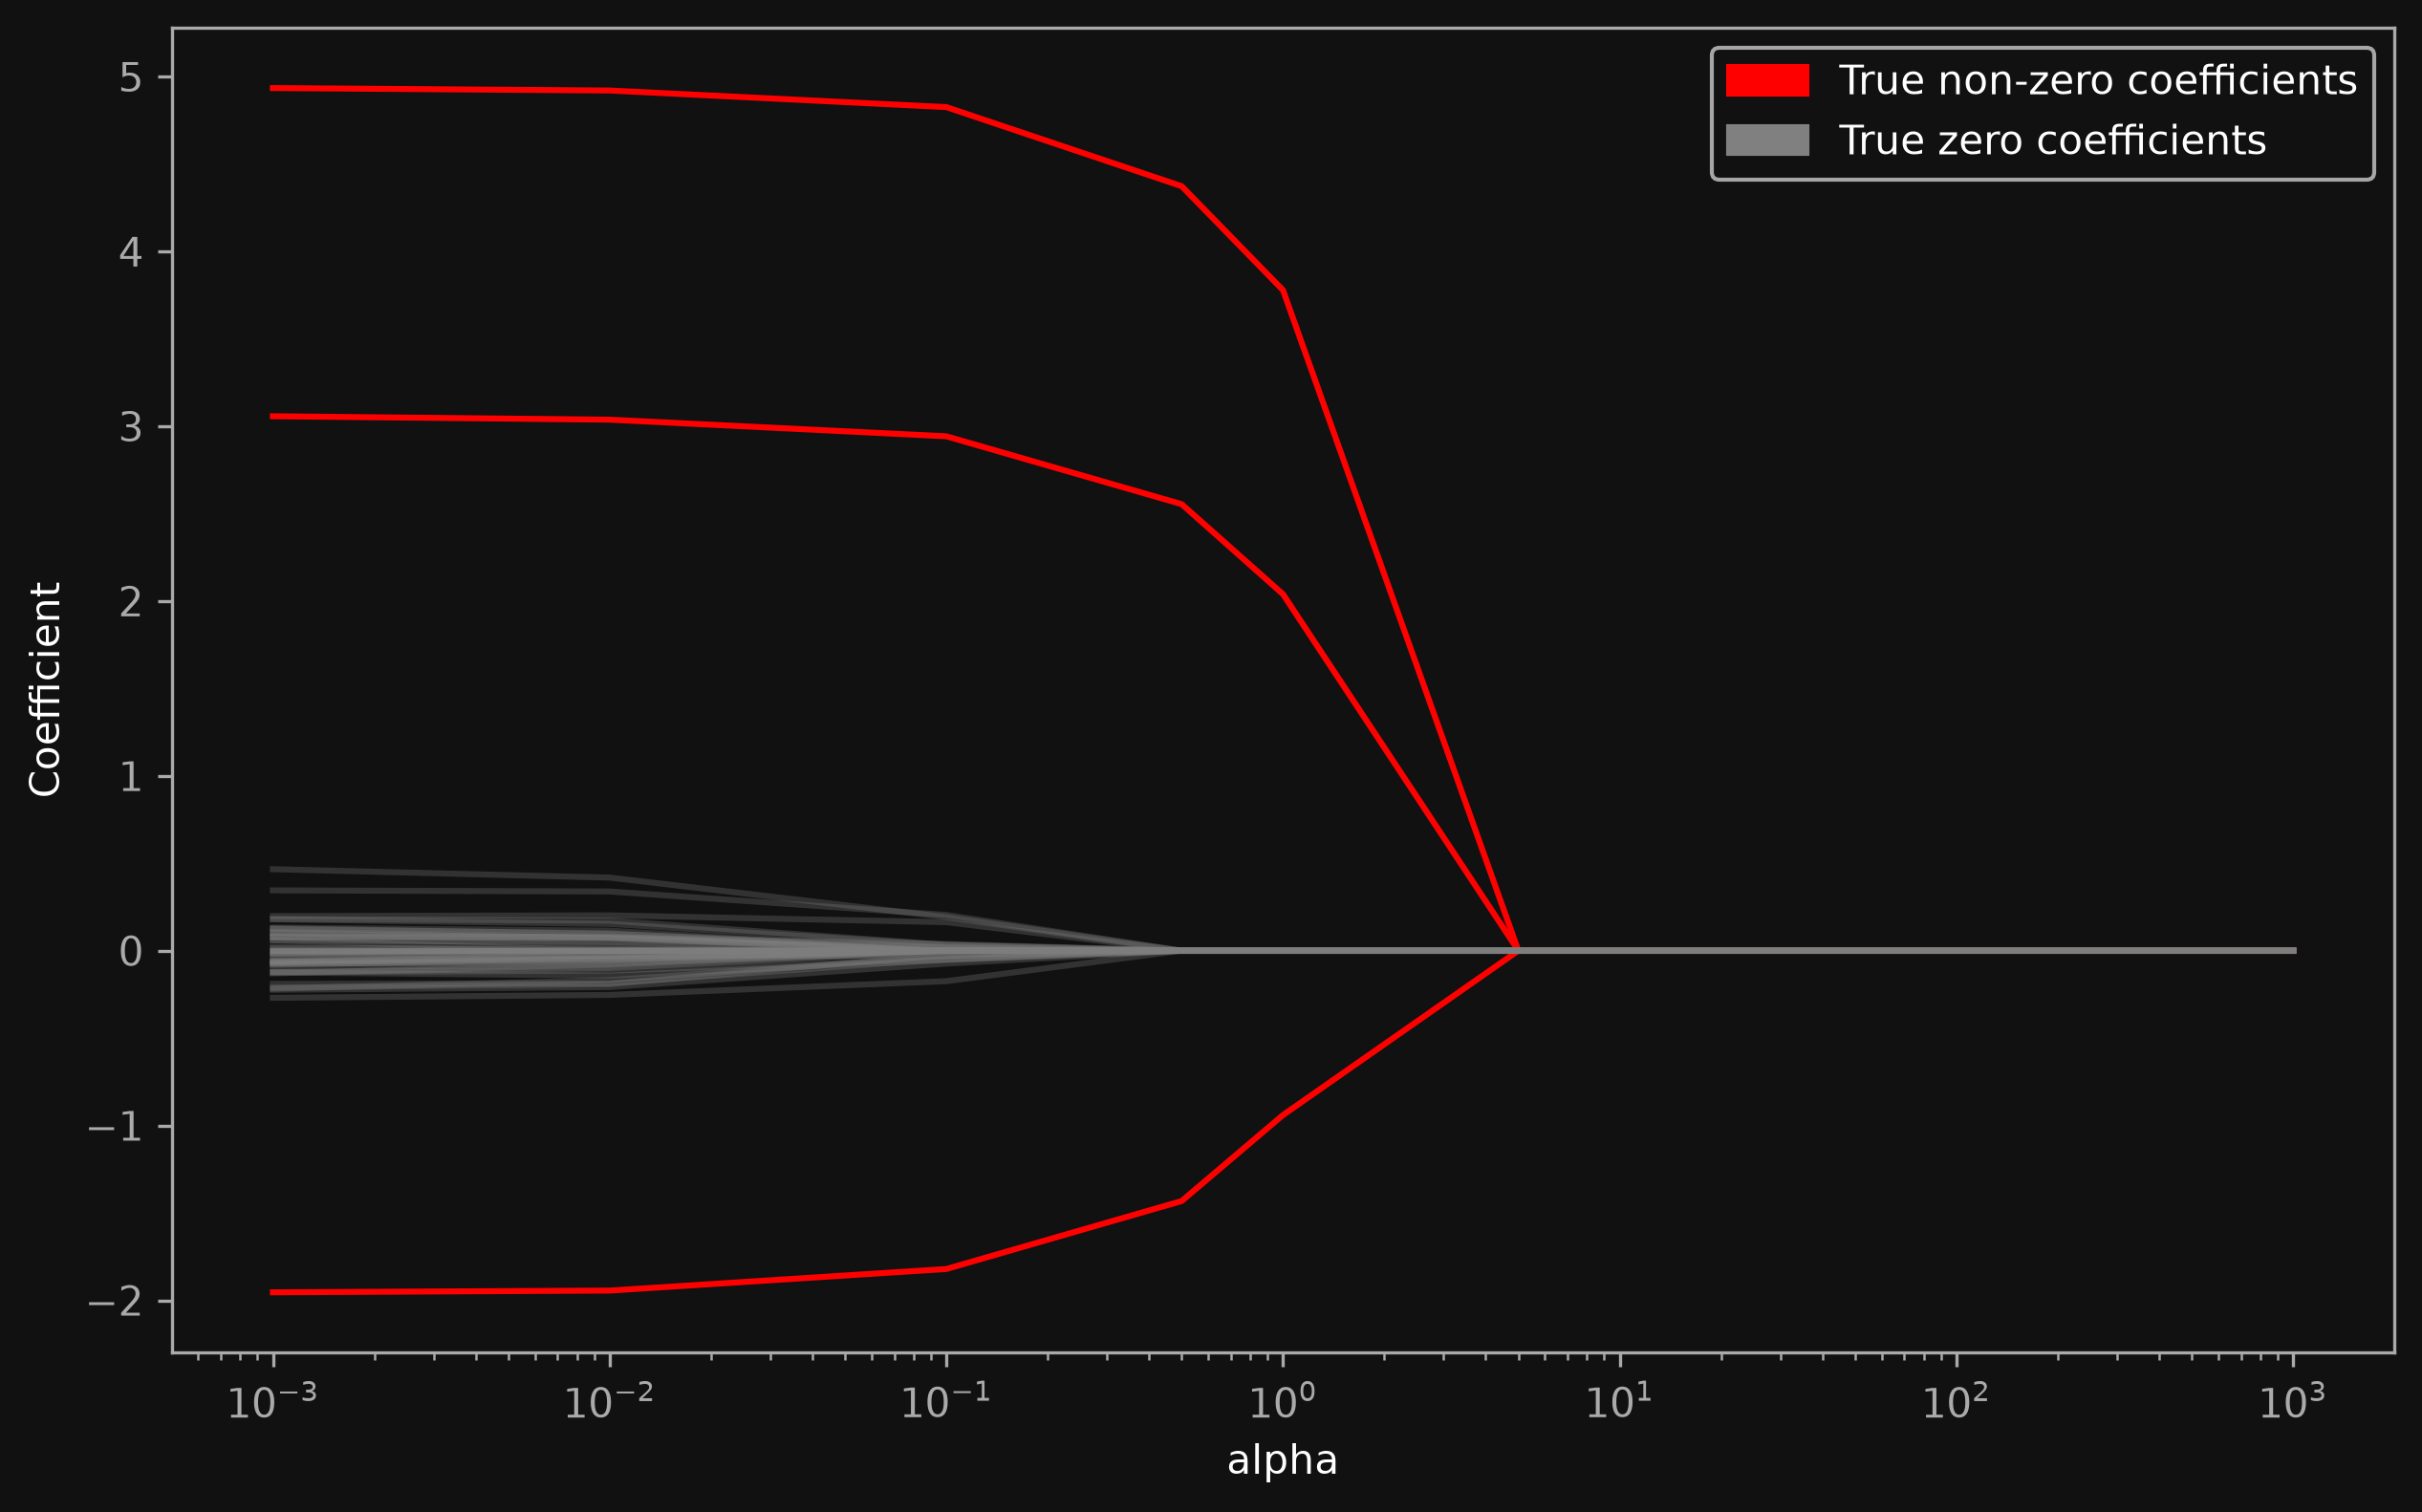
\includegraphics[width=0.68\textwidth]{./figures/problem2_lasso_path.png}
\end{center}

\begin{center}
\begin{tabular}{rrrr}
\toprule
$\alpha$ & $X_1$ (true 5) & $X_2$ (true $-2$) & $X_3$ (true 3) \\
\midrule
0.001 & 4.9344 & -1.9543 & 3.0572 \\
0.010 & 4.9204 & -1.9444 & 3.0375 \\
0.100 & 4.8256 & -1.8210 & 2.9424 \\
0.500 & 4.3733 & -1.4323 & 2.5543 \\
1.000 & 3.7783 & -0.9403 & 2.0392 \\
5.000 & 0.0000 & 0.0000 & 0.0000 \\
\bottomrule
\end{tabular}
\end{center}

The noise coefficients are gone by $\alpha \approx 1$; the real ones survive to somewhere between
$1$ and $5$. That gap is the window in which Lasso does feature selection.

The bias is a shift, not a scaling. Going from $\alpha = 0.001$ to $\alpha = 1$ moves $X_1$ by
$1.156$, $X_2$ by $1.014$ and $X_3$ by $1.018$ -- each coefficient loses roughly $\alpha$ in
absolute value, which is soft-thresholding. That is why the smallest true coefficient, $-2$, is the
worst hit in relative terms: it has lost $53\%$ of its size at $\alpha = 1$ while $X_1$ has lost
$24\%$. It is also why every coefficient hits zero at once here, rather than fading out.



\problem{3: Time Series and Time-Varying Heteroskedasticity}

Generate a dataset with $n=1000$ observations. 
The data follows an AR(1) process:
$$ y_t = 0.5 y_{t-1} + \epsilon_t $$
The error term $\epsilon_t$ follows an ARCH(1) process plus a regime:
$$ \epsilon_t = \sigma_t z_t, \quad z_t \sim \mathcal{N}(0,1) $$
$$ \sigma_t^2 = 1 + 0.5 \epsilon_{t-1}^2 + 10 \cdot \mathbb{I}_{\text{HighRegime}} $$

Use the following code snippet to generate your data:
    \begin{lstlisting}[language=Python]
import numpy as np
import pandas as pd

np.random.seed(100)
n = 1000

indicator = np.zeros(n)
for i in range(0, n, 200):
    indicator[i:i+100] = 1 

epsilon = np.zeros(n)
sigma2 = np.zeros(n)
epsilon[0] = np.random.normal(0, 1)

for t in range(1, n):
    sigma2[t] = 1 + 0.5 * (epsilon[t-1]**2) + 10 * indicator[t]
    epsilon[t] = np.random.normal(0, np.sqrt(sigma2[t]))

y = np.zeros(n)
phi = 0.5
for t in range(1, n):
    y[t] = phi * y[t-1] + epsilon[t]\end{lstlisting}

\subproblem{3.1: The AR(1) Model}

First, fit an AR(1) model to the generated series $y_t$.
$$
y_t = \phi y_{t-1} + \epsilon_t
$$

Extract the residuals $\epsilon_t$ from this model.

Create two plots:
\begin{itemize}
    \item Residuals vs. fitted values.
    \item Residuals over time.
\end{itemize}
What do you notice about the first graph vs. the second graph?

\answer
$\hat{\phi} = 0.5182$ against a true $0.5$, so the conditional mean is recovered.

\begin{center}
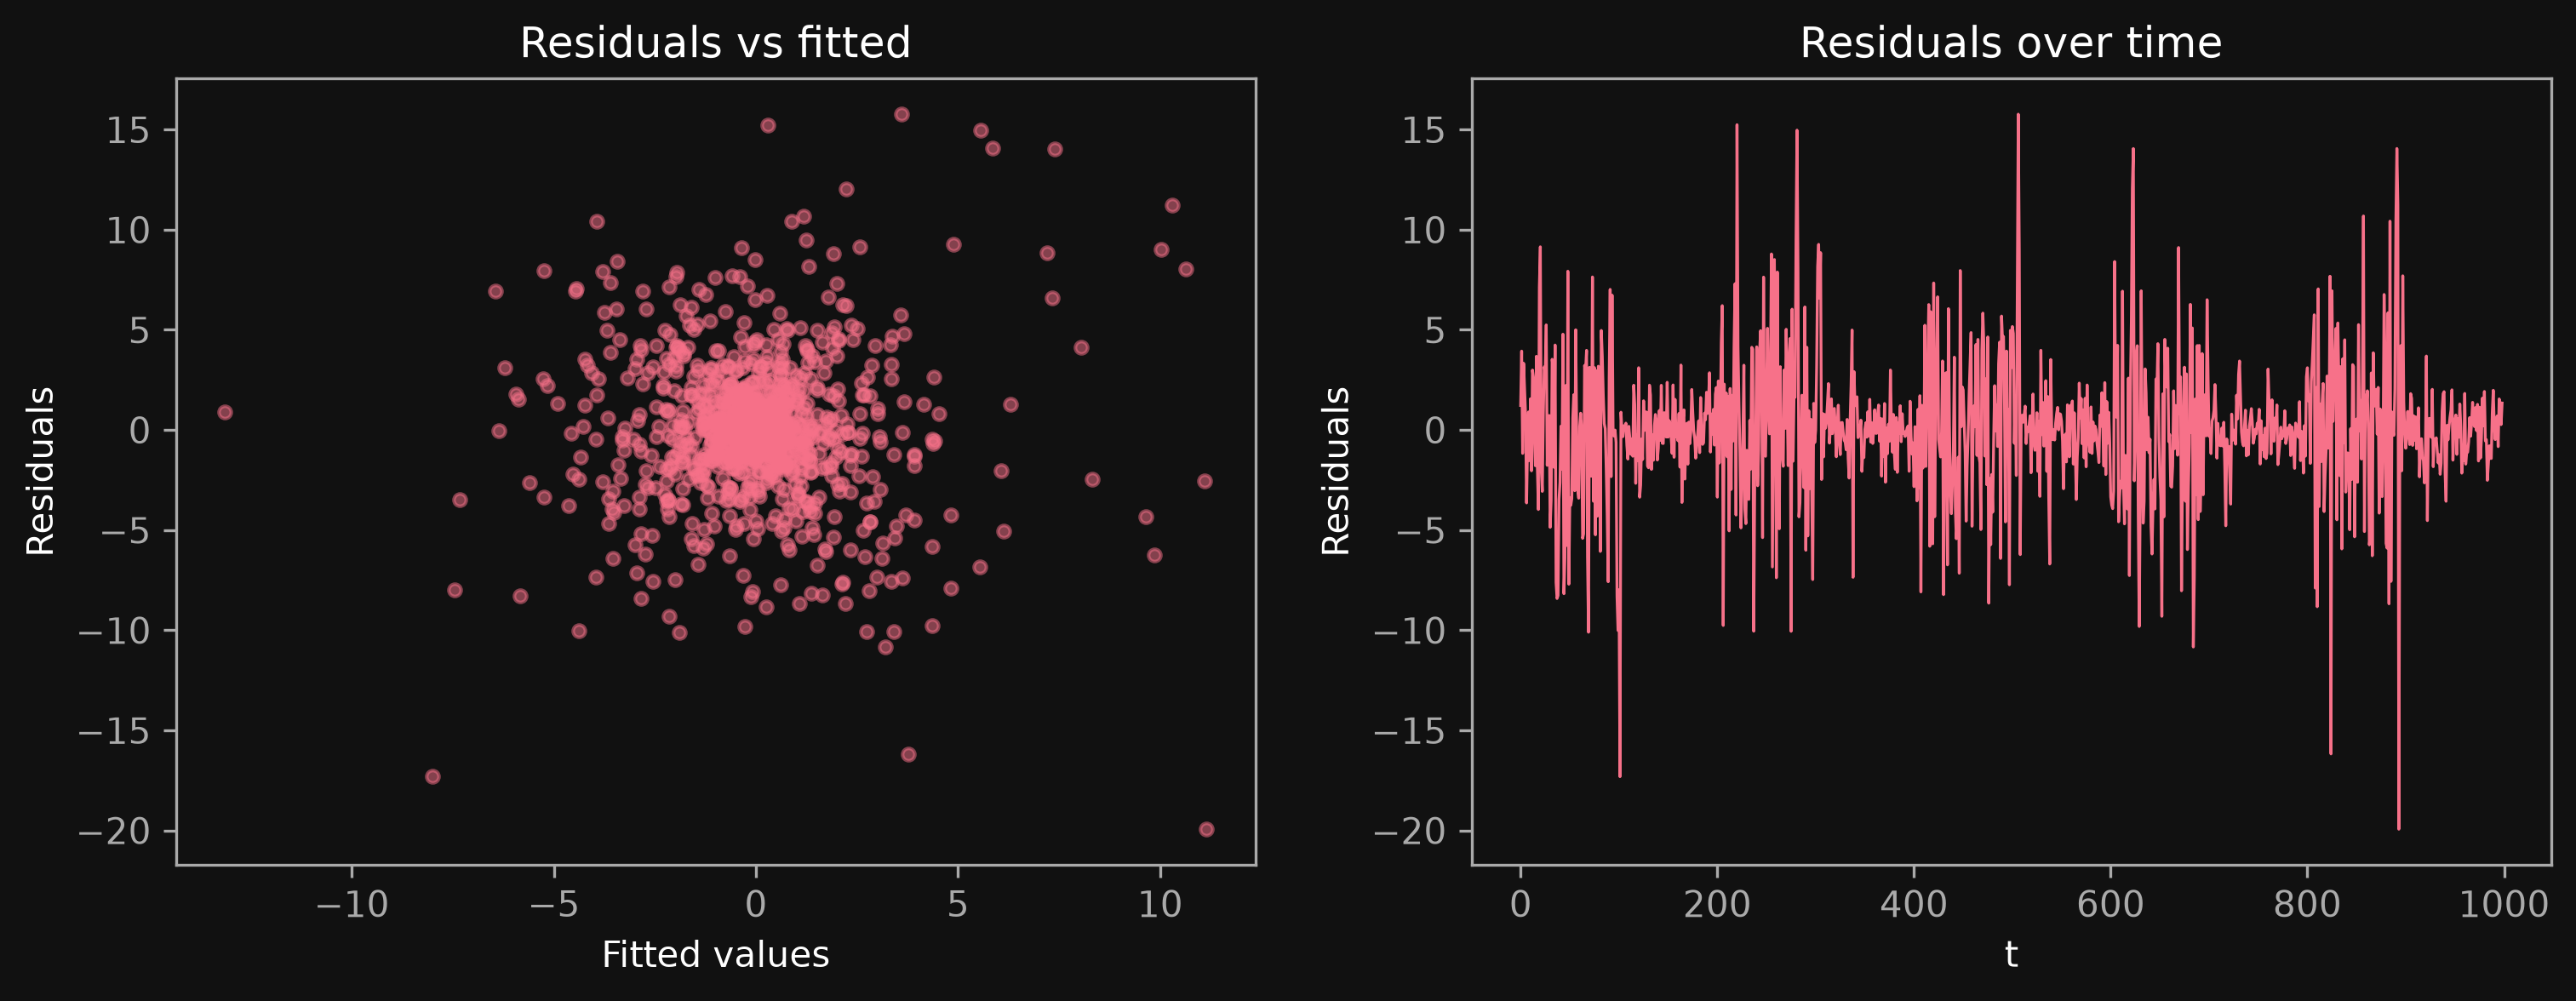
\includegraphics[width=0.95\textwidth]{./figures/problem3_ar1_residuals.png}
\end{center}

Residuals versus fitted values shows nothing: an even band, no funnel, no curvature. That plot is
blind here, because it sorts the residuals by fitted value and the variance does not depend on the
fitted value.

Residuals over time shows everything: alternating stretches of wild and quiet, on a period of about
200 steps. The variance depends on $t$, not on $\hat{y}$, so ordering the residuals by time is the
only way to see it.


\subproblem{3.2: ACF}
Plot the Autocorrelation Function (ACF) of the squared residuals $\hat{\epsilon}_t^2$.

What does the ACF plot suggest about the independence of the squared residuals?

\answer
\begin{center}
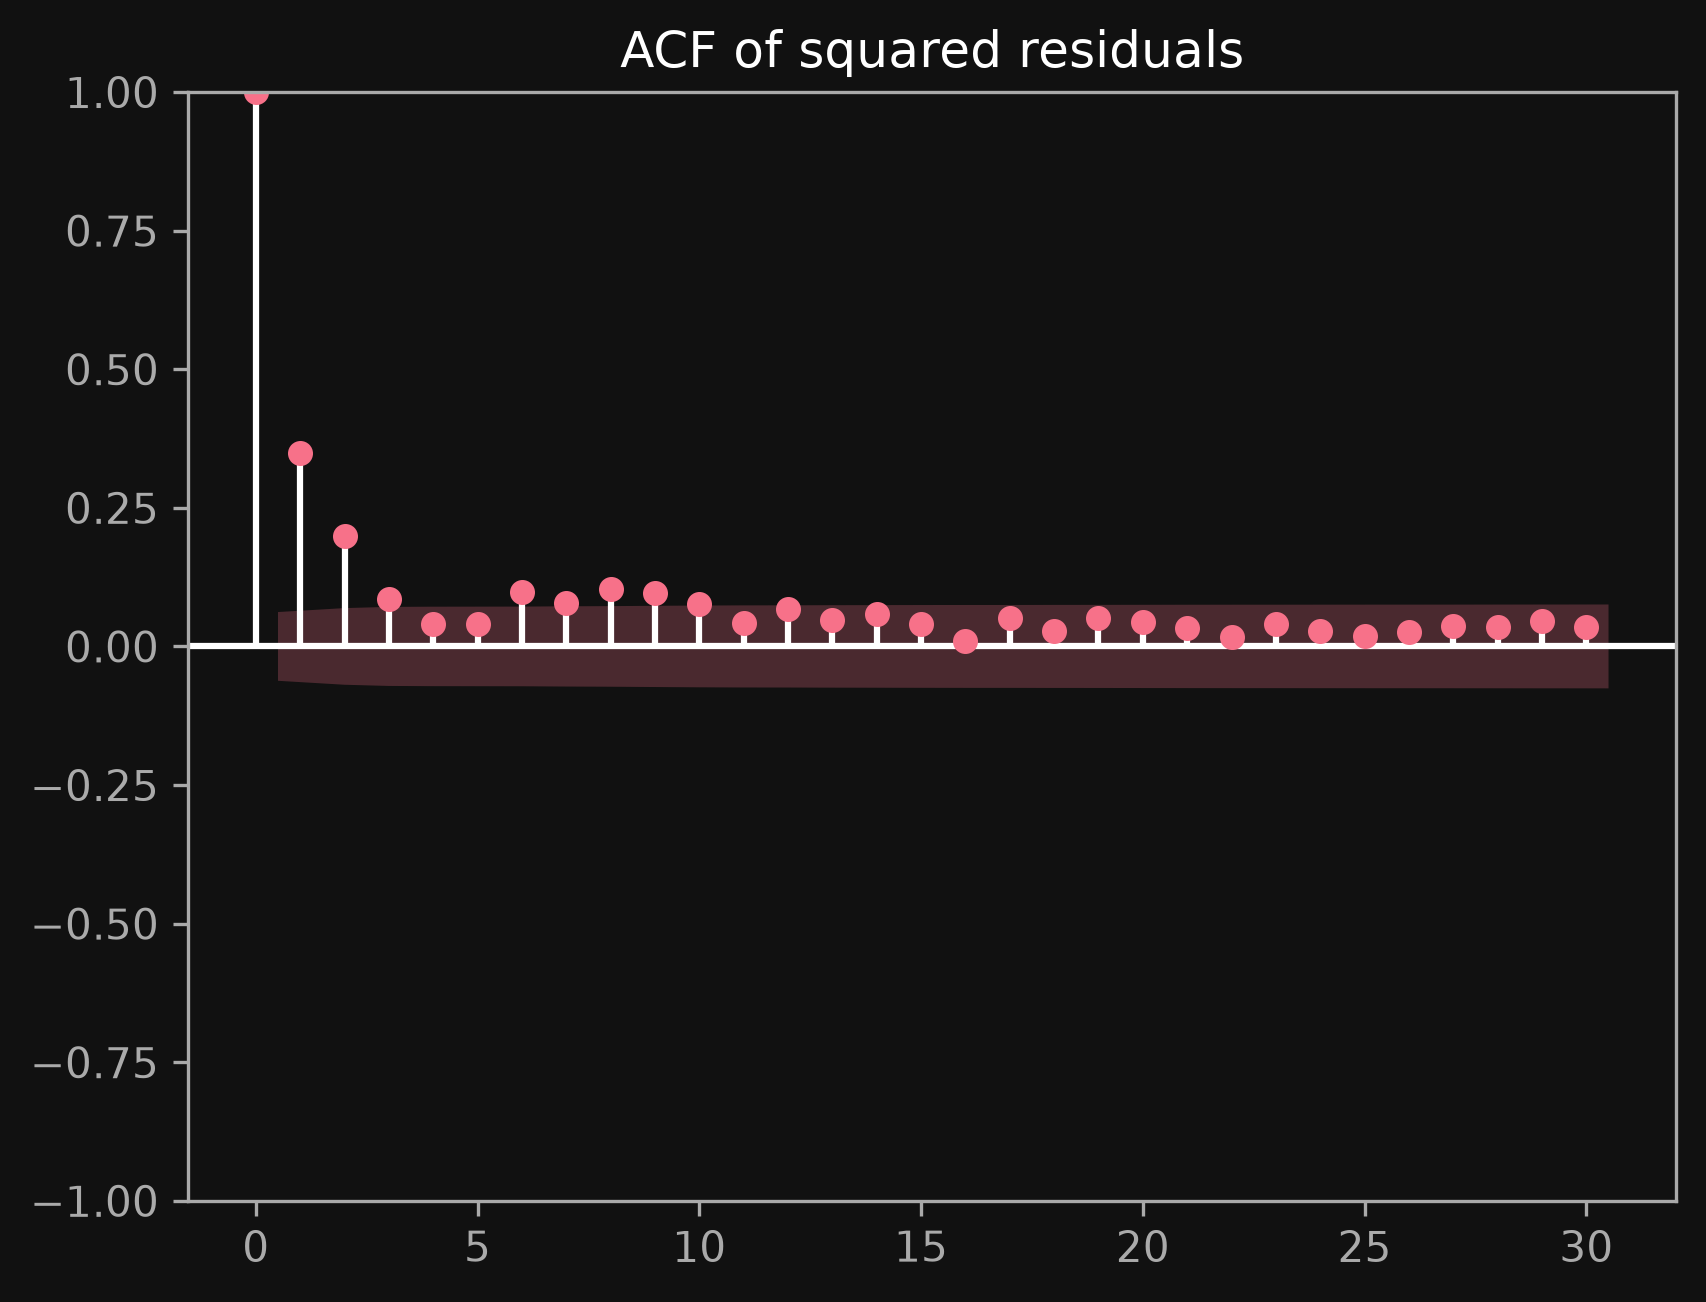
\includegraphics[width=0.58\textwidth]{./figures/problem3_acf_squared_residuals.png}
\end{center}

The squared residuals are strongly autocorrelated: the first several lags sit well outside the
confidence band, and the decay is slow.

The residuals themselves are uncorrelated -- the AR(1) took care of that -- but their squares are
not, so the residuals are not independent. A big move today predicts a big move tomorrow, in
magnitude but not in sign. That is volatility clustering, and it is exactly what the ARCH term plus
the regime put into the data.


\subproblem{3.3: Modeling Variance (ARCH + Regime)}
Now, we will model the variance of these residuals explicitly. We hypothesize that the variance $\sigma_t^2$ depends on the previous squared residual (ARCH effect) and the regime indicator.
\begin{itemize}
    \item Construct the squared residuals $\hat{\epsilon}_t^2$.
    \item Construct a lagged feature $\hat{\epsilon}_{t-1}^2$.
    \item Run a linear regression of $\hat{\epsilon}_t^2$ on:
    $$ \sigma_t^2 = \beta_0 + \beta_1 \hat{\epsilon}_{t-1}^2 + \beta_2 \mathbb{I}_{\text{HighRegime}} $$
    \item Report the coefficients, compare them to the true values ($\beta_0=1$, $\beta_1=0.5$, $\beta_2=10$), and discuss their statistical significance.
\end{itemize}

\answer
\begin{center}
\begin{tabular}{lcccccc}
\toprule
                      & \textbf{coef} & \textbf{std err} & \textbf{t} & \textbf{P$> |$t$|$} & \textbf{[0.025} & \textbf{0.975]}  \\
\midrule
\textbf{const}        &       2.9868  &        1.233     &     2.422  &         0.016        &        0.567    &        5.406     \\
\textbf{resid2\_lag1} &       0.2994  &        0.030     &     9.927  &         0.000        &        0.240    &        0.359     \\
\textbf{indicator}    &      11.3243  &        1.795     &     6.307  &         0.000        &        7.801    &       14.848     \\
\bottomrule
\end{tabular}
\end{center}

All three are significant, and both the ARCH term and the regime dummy overwhelmingly so
($t = 9.93$ and $t = 6.31$). The regression finds the right structure.

The point estimates are only roughly right: $2.9868$ against $\beta_0 = 1$, $0.2994$ against
$\beta_1 = 0.5$, $11.3243$ against $\beta_2 = 10$. The ARCH coefficient is the one that is clearly
off, and the intercept absorbs what it gives up. Two reasons: $\hat{\epsilon}_{t-1}^2$ is a noisy
proxy for $\epsilon_{t-1}^2$, which attenuates $\hat{\beta}_1$ toward zero in the usual
errors-in-variables way; and $\hat{\epsilon}_t^2$ is an extremely skewed dependent variable, so OLS
on it is inefficient and its coefficients are unstable in a sample of 998.


\subproblem{3.4: Regime-Dependent Forecasting}
Suppose we are at the end of the series ($T=1000$) and we want to predict the range of movement for the next step ($T=1001$).
Assume the last observed residual was $\hat{\epsilon}_{1000} = 2$.

Calculate the predicted variance $\hat{\sigma}_{1001}^2$ and the resulting 95\% Confidence Interval width ($\pm 1.96 \hat{\sigma}_{1001}$) for the error term under two scenarios:
\begin{itemize}
    \item \textbf{Scenario A (Low Regime):} Assume the indicator for $T=1001$ is 0.
    \item \textbf{Scenario B (High Regime):} Assume the indicator for $T=1001$ is 1.
\end{itemize}
(Use the coefficients you estimated in 3.3).

What do you observe about your confidence intervals in the two scenarios?

\answer
With $\hat{\epsilon}_{1000} = 2$, so $\hat{\epsilon}_{1000}^2 = 4$:
$$
\hat{\sigma}_{1001}^2 = 2.9868 + 0.2994 \times 4 + 11.3243 \times \mathbb{I}.
$$

\begin{center}
\begin{tabular}{lrrr}
\toprule
 & $\hat{\sigma}^2_{1001}$ & Lower Bound & Upper Bound \\
\midrule
Low Regime & 4.1846 & -4.0094 & 4.0094 \\
High Regime & 15.5088 & -7.7187 & 7.7187 \\
\bottomrule
\end{tabular}
\end{center}

The same model, the same last observation, and the interval is $1.93$ times wider in the high
regime. Nothing about the point forecast changed -- only the regime flag.

A single unconditional interval would be wrong in both directions at once: too wide in the quiet
regime and too narrow in the loud one, which is the worse of the two errors.


\problem{4: Weighted Least Squares}

This problem focuses on verifying the findings of Class 3 regarding
Weighted Least Squares (WLS).

\subproblem{4.1: Setup}

Similar to before, define the true model as:
$$
y = 2x
$$
Where $x$ is sampled from the uniform distribution $x \sim \text{Uniform}(1, 2)$.

Second, define the noise $\epsilon_i$ to be sampled from a normal distribution with mean 0,
and variance $\sigma_i^2$ that depends on $x_i$ as follows:
$$
\sigma_i^2 = \frac{1}{x_i^2}
$$

For $n=500$, please plot the generated data points $(x_i + \epsilon_i, y_i)$.

\answer
The true model has no intercept, so every fit below is through the origin, and the noise enters the
response: $y_i = 2 x_i + \epsilon_i$ with $\epsilon_i \sim \mathcal{N}(0,\, 1/x_i^2)$. That is what
makes $w_i = x_i^2$ the correct GLS weights in 4.5, since $w_i = 1/\sigma_i^2$.

\begin{lstlisting}[language=Python]
np.random.seed(500)
n = 500

x = np.random.uniform(1, 2, n)
sigma = 1 / x
epsilon = np.random.normal(0, sigma)
y = 2 * x + epsilon
\end{lstlisting}

\begin{center}
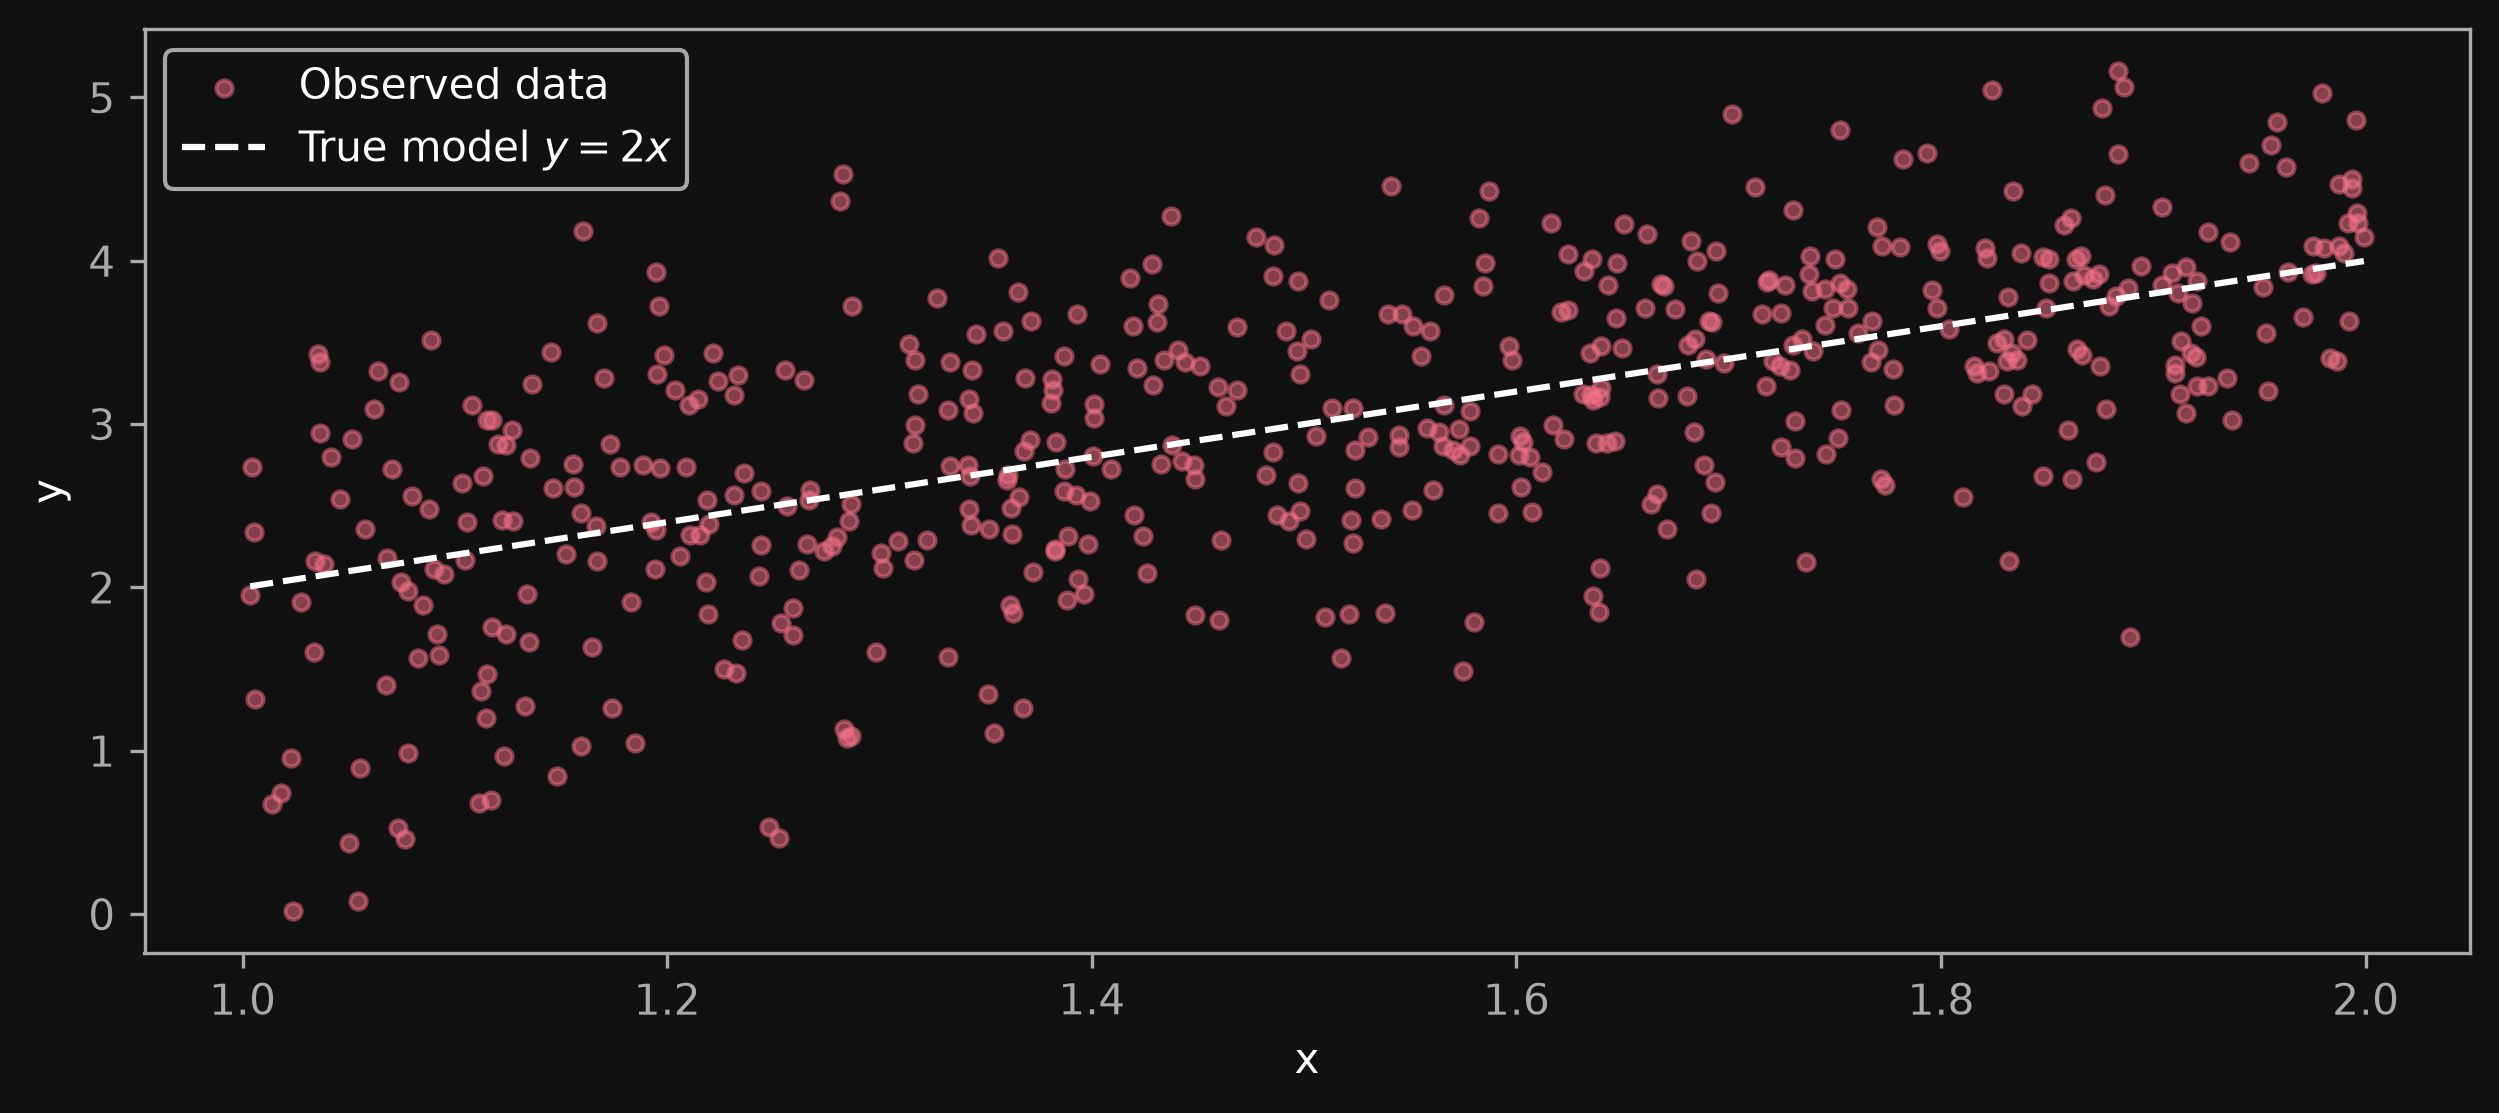
\includegraphics[width=0.95\textwidth]{./figures/problem4_scatter.png}
\end{center}

The vertical spread is widest at $x = 1$ ($\sigma_i = 1$) and narrowest at $x = 2$
($\sigma_i = 1/2$), which is the heteroskedasticity we built in.


\subproblem{4.2: Naive OLS}

Fit a standard OLS regression to the data generated above.

Report your estimate $\hat{\beta}_{\text{OLS}}$, and the confidence interval for the estimate.

\answer
\begin{center}
\begin{tabular}{lcccccc}
\toprule
            & \textbf{coef} & \textbf{std err} & \textbf{t} & \textbf{P$> |$t$|$} & \textbf{[0.025} & \textbf{0.975]}  \\
\midrule
\textbf{x}  &       1.9975  &        0.021     &    96.001  &         0.000        &        1.957    &        2.038     \\
\bottomrule
\end{tabular}
\end{center}

$\hat{\beta}_{\text{OLS}} = 1.9975$, with a 95\% interval of $[1.9566,\, 2.0384]$. The point estimate
is fine -- OLS is still unbiased under heteroskedasticity. What is wrong is the standard error.


\subproblem{4.3: Interpretation}

Briefly discuss whether naive OLS will be under or over confident in its estimate of $\hat{\beta}_{\text{OLS}}$,
and why.

\answer
\textbf{Under-confident}: the reported interval is wider than it needs to be.

For a fit through the origin, $\hat{\beta} - \beta = \sum_i x_i \epsilon_i / \sum_i x_i^2$, so the
true variance is
$$
\Var(\hat{\beta}_{\text{OLS}}) = \frac{\sum_i x_i^2 \sigma_i^2}{\left(\sum_i x_i^2\right)^2}
= \frac{\sum_i x_i^2 \cdot (1/x_i^2)}{\left(\sum_i x_i^2\right)^2}
= \frac{n}{\left(\sum_i x_i^2\right)^2},
$$
whereas OLS \textit{reports} $\bar{\sigma}^2 / \sum_i x_i^2$, charging every point one common
variance. The ratio of reported to true variance is
$$
\frac{\bar{\sigma}^2 \sum_i x_i^2}{n} \;\longrightarrow\;
\E\!\left[\tfrac{1}{x^2}\right] \E\!\left[x^2\right] = \frac{1}{2} \cdot \frac{7}{3} = \frac{7}{6},
$$
so the reported standard error is about $\sqrt{7/6} \approx 1.08$ times too large.

In a fit through the origin the large-$x$ points carry the most weight, and those are exactly the
points with the \textit{smallest} noise, since $\sigma_i = 1/x_i$. OLS charges them the average
noise level instead, so it overstates its own uncertainty. The heteroskedasticity-robust (HC3)
standard errors from Class 2 confirm it:

\begin{center}
\begin{tabular}{lrrrr}
\toprule
 & $\hat{\beta}$ & std err & CI lower & CI upper \\
\midrule
OLS (conventional) & 1.99752 & 0.02081 & 1.95664 & 2.03840 \\
OLS (HC3 robust)   & 1.99752 & 0.01962 & 1.95907 & 2.03596 \\
\bottomrule
\end{tabular}
\end{center}

The realized ratio of the two standard errors is $1.0608$, against the $1.0801$ the algebra
predicts in the limit.

Note that the direction is specific to this design. If the variance \textit{grew} with $x$ instead,
the heavily weighted points would be the noisy ones and naive OLS would be over-confident.


\subproblem{4.4: Visualization}

Plot a Q-Q plot of the residuals from the naive OLS regression. What do you observe?

\answer
\begin{center}
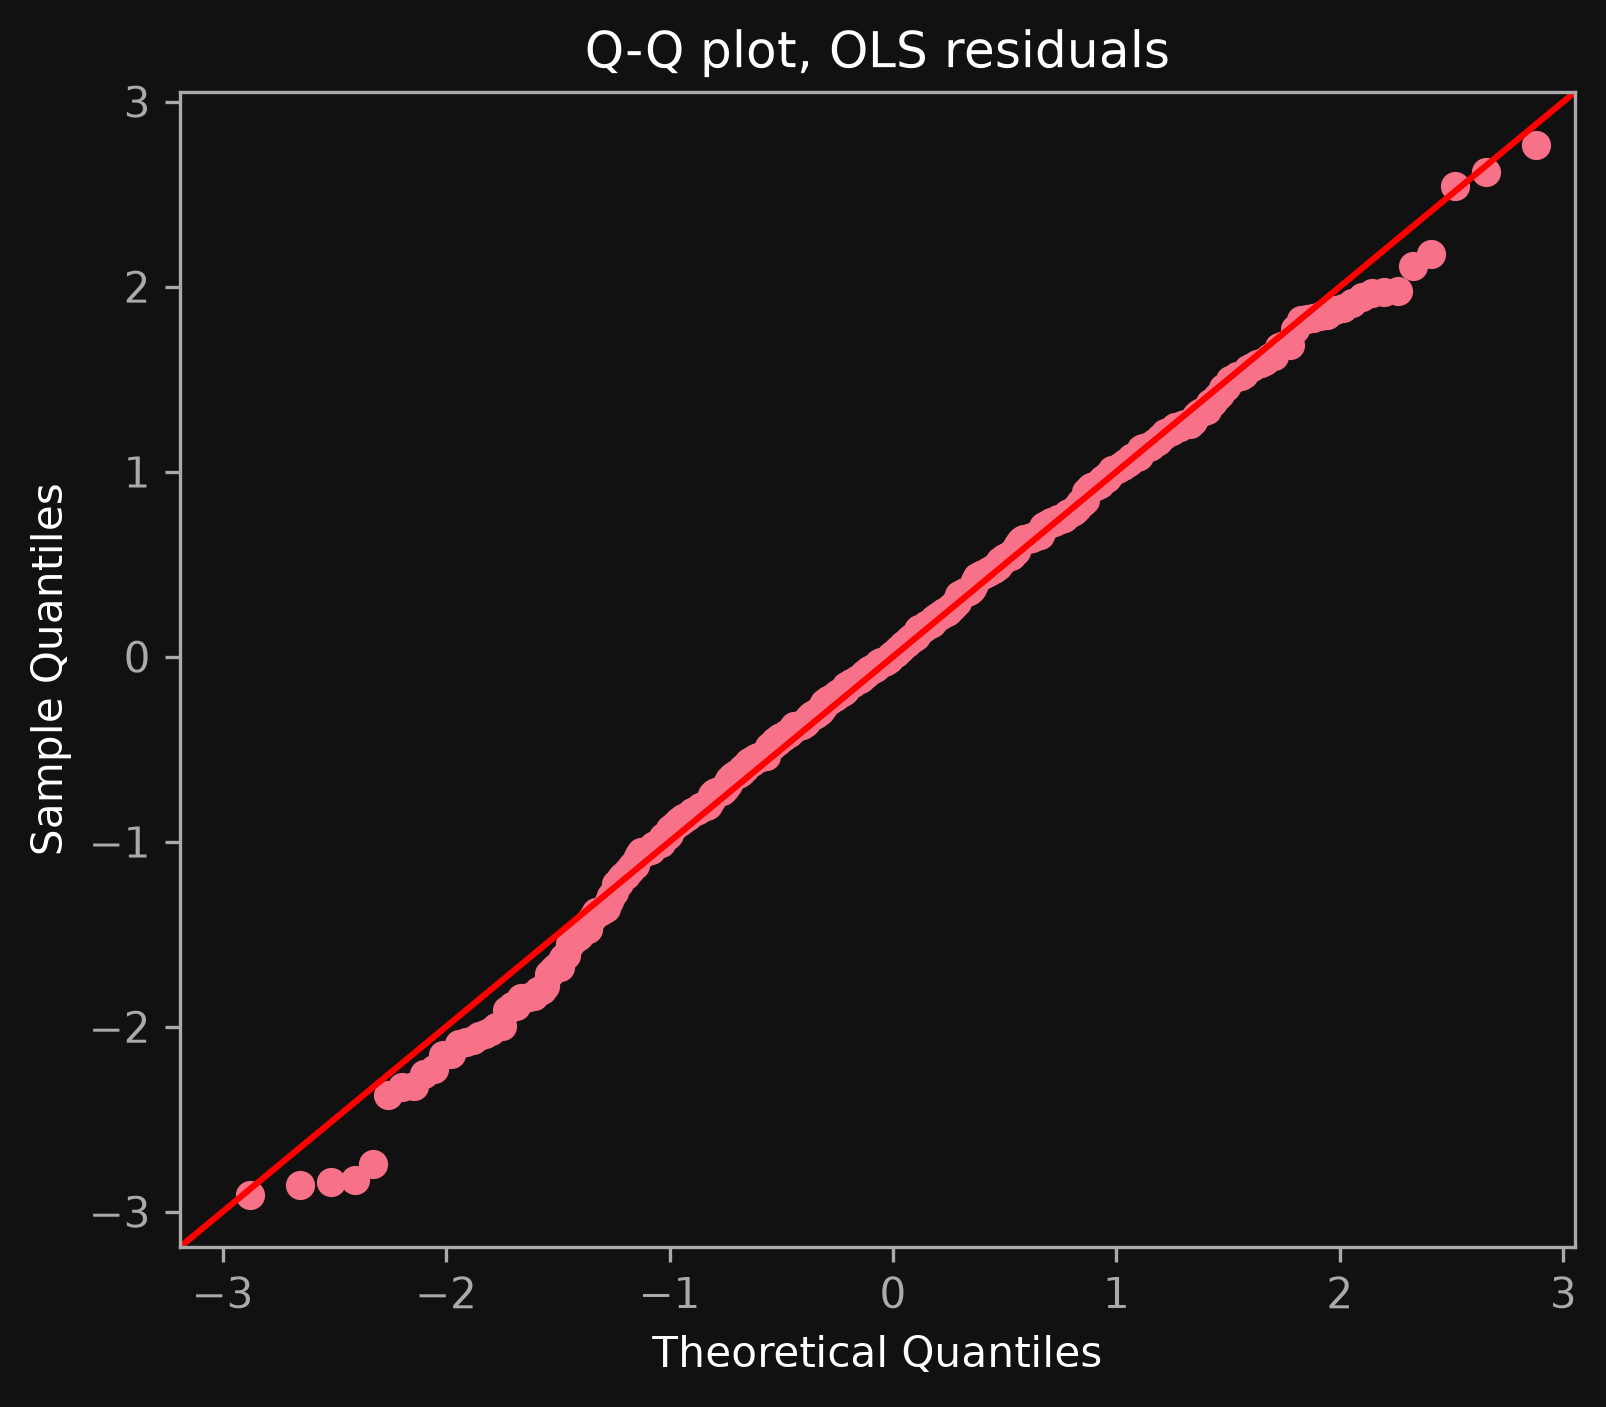
\includegraphics[width=0.58\textwidth]{./figures/problem4_qq_ols.png}
\end{center}

The points bend away from the $45^\circ$ line in both tails. Each $\epsilon_i$ is normal on its own,
but the residuals pool draws from 500 \textit{different} variances -- a scale mixture of normals,
which is not itself normal. Shapiro-Wilk gives $p = 0.0482$, which rejects at the $5\%$ level.


\subproblem{4.5: Weighted Least Squares}

Fit a Weighted Least Squares regression to the data generated above, using weights $w_i = x_i^2$.
Report your estimate $\hat{\beta}_{\text{WLS}}$, and the confidence interval for the estimate.

\answer
\begin{center}
\begin{tabular}{lcccccc}
\toprule
            & \textbf{coef} & \textbf{std err} & \textbf{t} & \textbf{P$> |$t$|$} & \textbf{[0.025} & \textbf{0.975]}  \\
\midrule
\textbf{x}  &       2.0024  &        0.018     &   108.781  &         0.000        &        1.966    &        2.039     \\
\bottomrule
\end{tabular}
\end{center}

$\hat{\beta}_{\text{WLS}} = 2.0024$, with a 95\% interval of $[1.966,\, 2.039]$. The weights
$w_i = x_i^2 = 1/\sigma_i^2$ are exactly the GLS weights, so by Gauss-Markov this is the efficient
estimator: its standard error of $0.018$ beats both the conventional and the robust OLS numbers
from 4.3.


\subproblem{4.6: Visualization}

Plot a Q-Q plot of the weighted residuals from the WLS regression. What do you observe compared
to the Q-Q plot from the naive OLS regression?

\answer
\begin{center}
\begin{minipage}{0.48\textwidth}
    \centering
    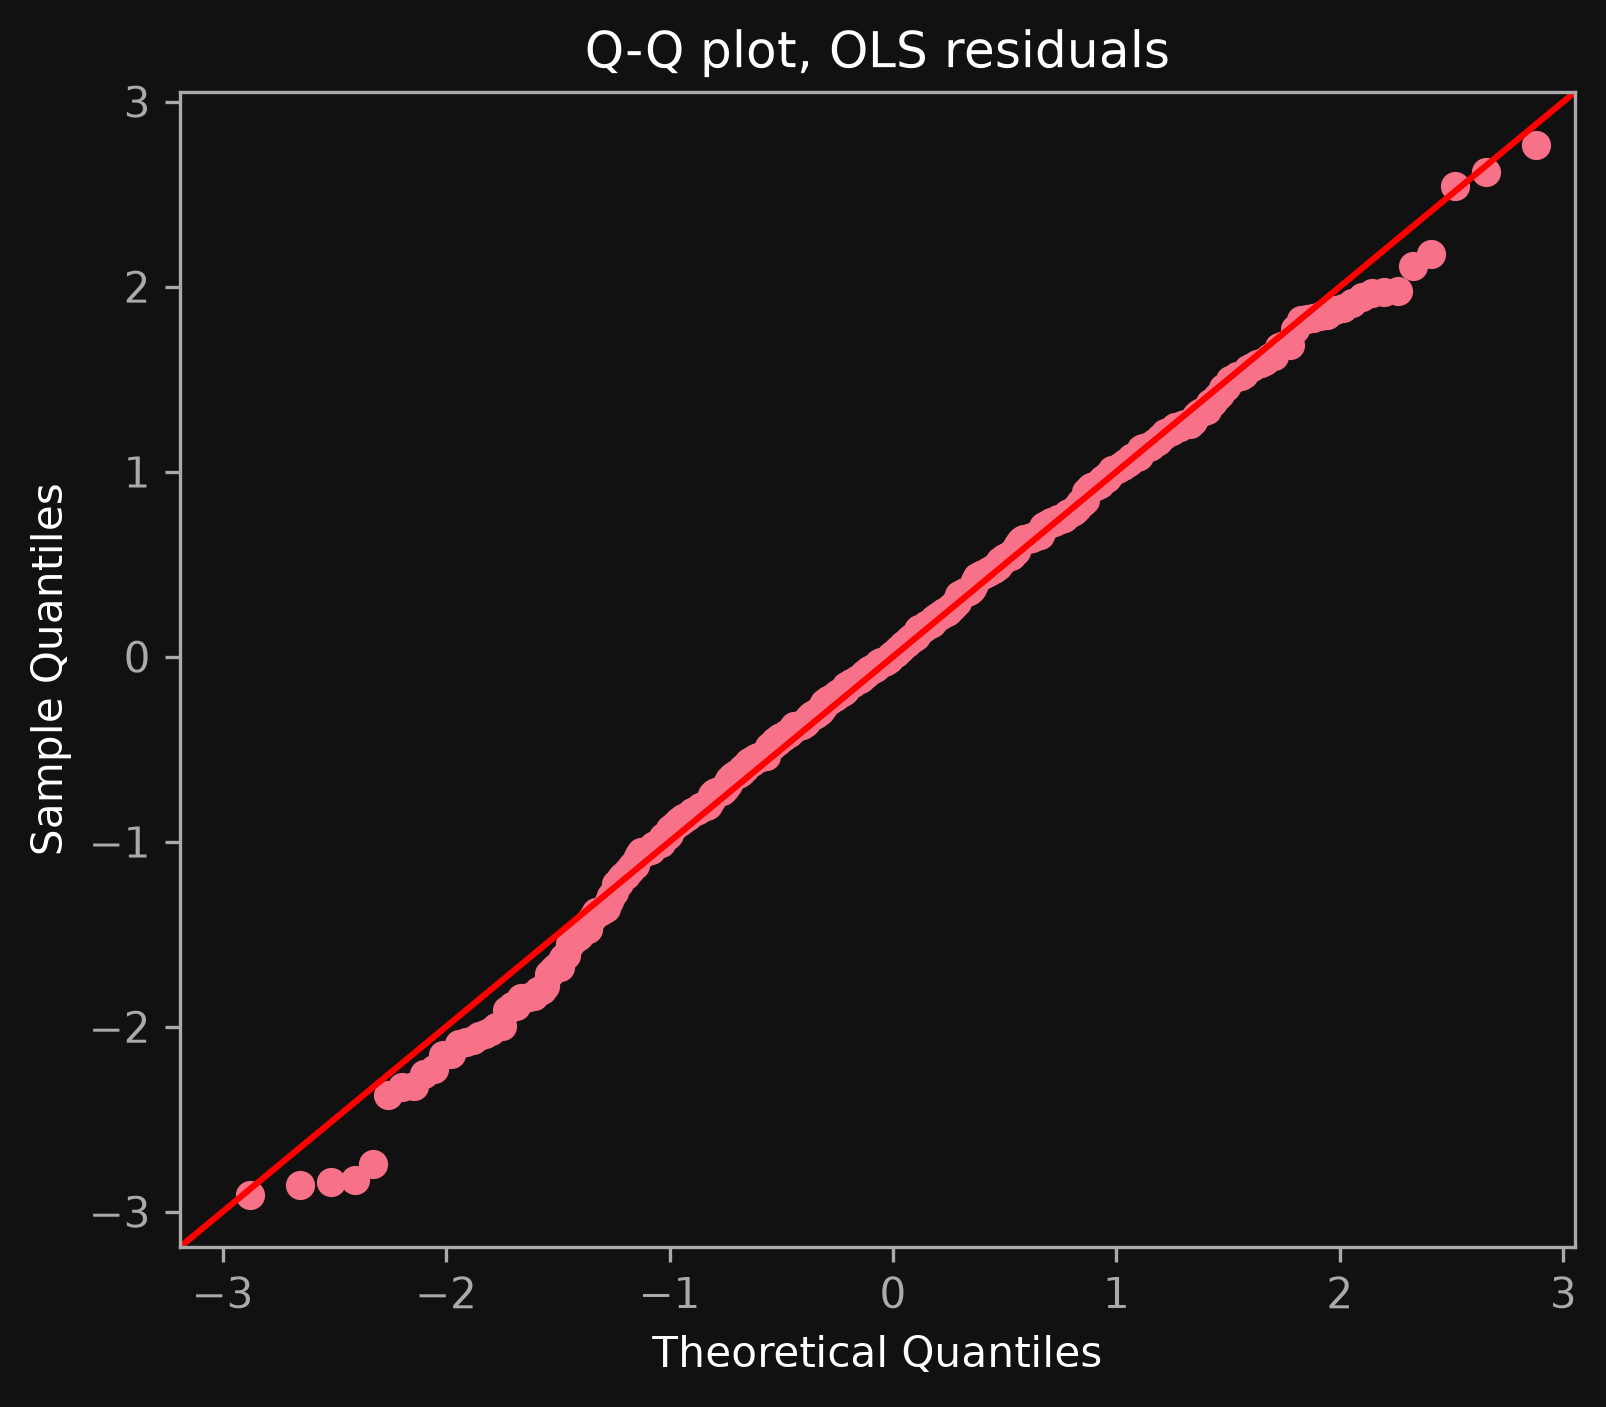
\includegraphics[width=\textwidth]{./figures/problem4_qq_ols.png}\\[3pt]
    Naive OLS
\end{minipage}
\hfill
\begin{minipage}{0.48\textwidth}
    \centering
    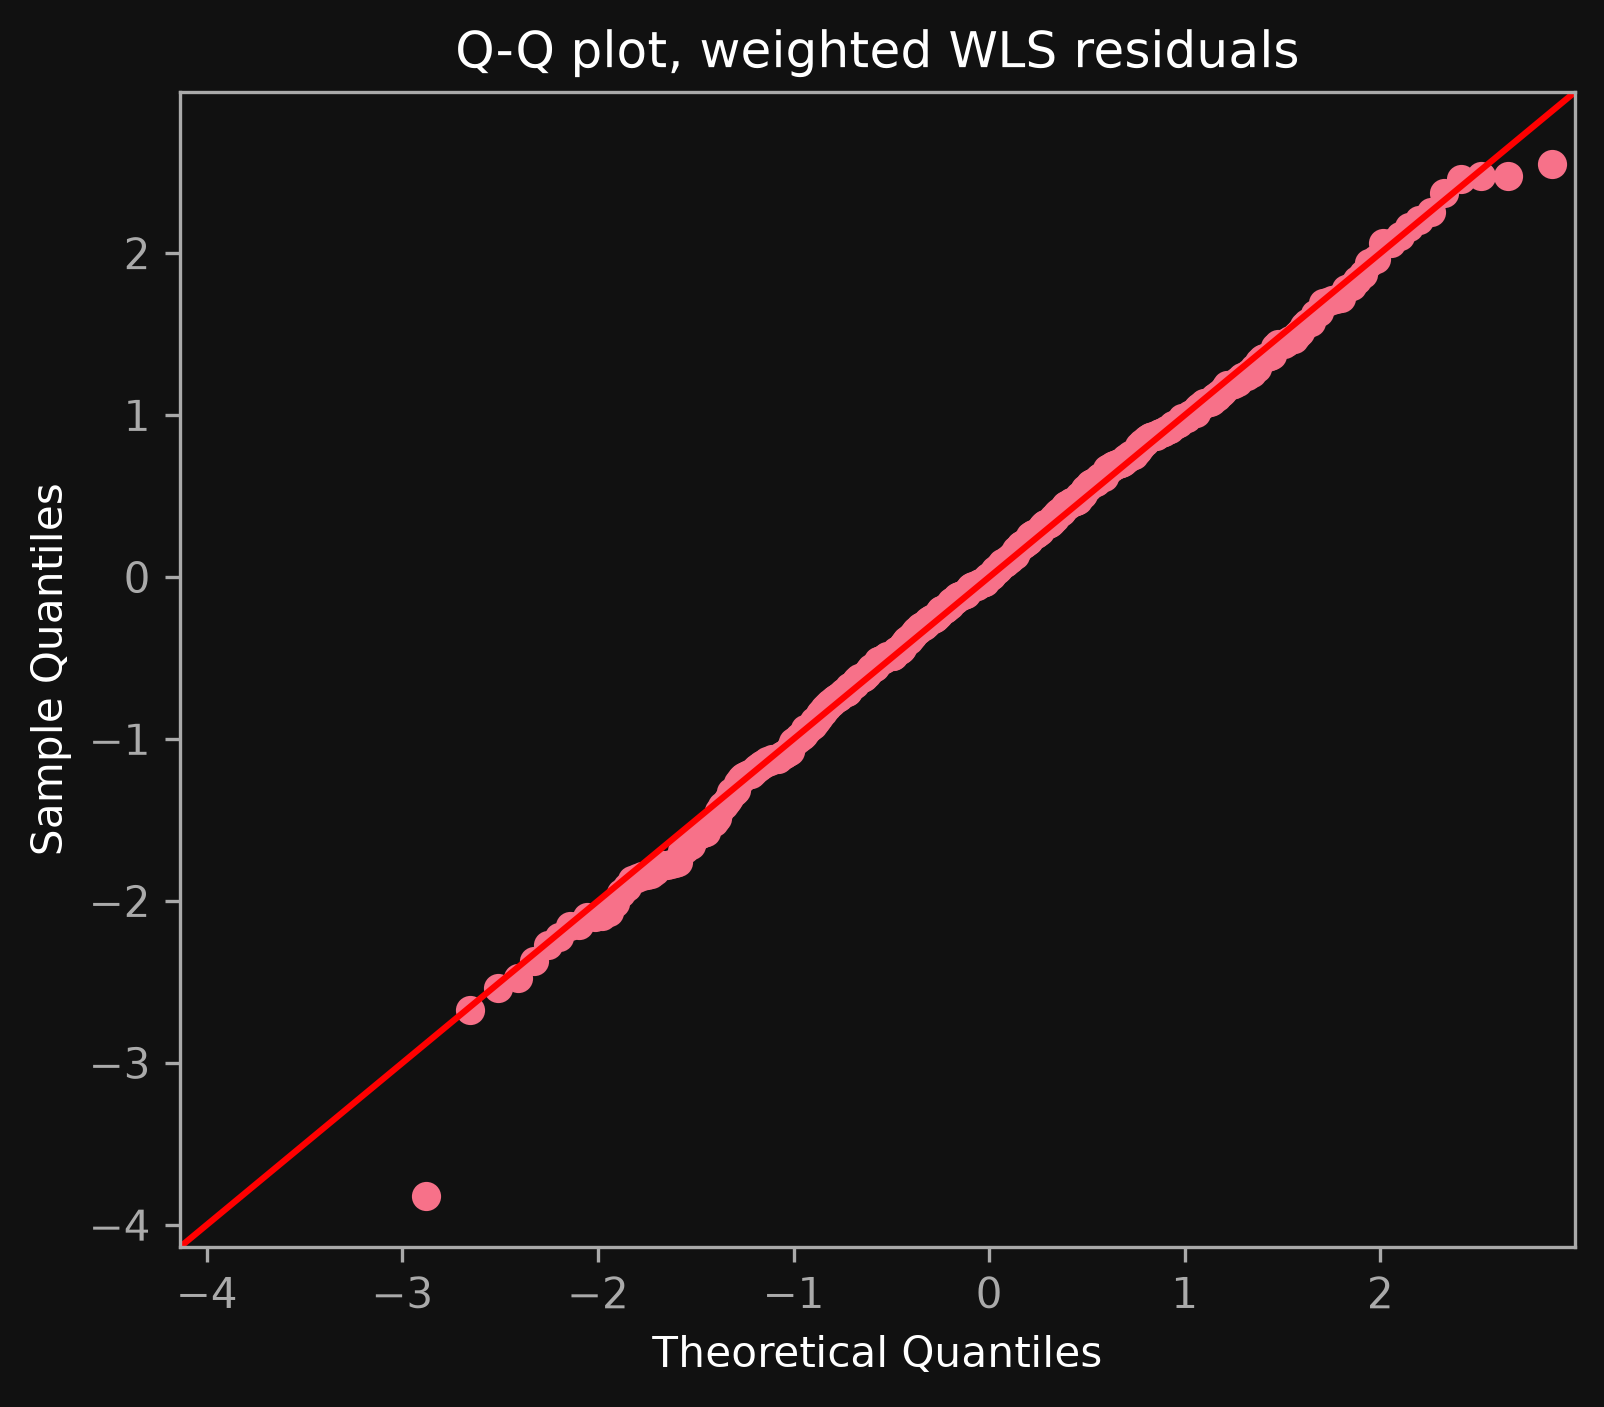
\includegraphics[width=\textwidth]{./figures/problem4_qq_wls.png}\\[3pt]
    WLS, weighted residuals
\end{minipage}
\end{center}

Much straighter, and the reason is exact: the weighted residual is
$\sqrt{w_i}\, \epsilon_i = x_i \epsilon_i$, which has variance $x_i^2 \cdot (1/x_i^2) = 1$ for
\textit{every} $i$. Weighting turns the scale mixture back into a single standard normal.

\begin{center}
\begin{tabular}{lrrr}
\toprule
 & std dev & Shapiro $p$ & corr($|\hat{\epsilon}|$, $x$) \\
\midrule
OLS residuals            & 0.7128 & 0.0482 & -0.2224 \\
Weighted (WLS) residuals & 1.0293 & 0.3125 & \phantom{-}0.0292 \\
\bottomrule
\end{tabular}
\end{center}

The weighted residuals have a sample standard deviation of $1.0293$ against a theoretical $1$,
Shapiro-Wilk no longer rejects, and the correlation between $|\hat{\epsilon}_i|$ and $x_i$ has
collapsed from $-0.2224$ to $0.0292$.

Note that \texttt{model\_wls.resid} returns the \textit{raw} residuals $y_i - x_i \hat{\beta}$,
which are still heteroskedastic. The weighted ones are \texttt{model\_wls.wresid}.



\end{document}